\section{Część realizująca sterowanie bezpośrednie (,,niższego poziomu'')}
\label{sec:czesc-nizsza}

Ze względu na dostępność sprzętu służącego do sterowania fizycznym układem zbiorników, wybór technologii mogącej stanowić podstawę niższego poziomu aplikacji był ograniczony do dwóch możliwości.

Stanowisko laboratoryjne jest wyposażone w komputer, który za pomocą karty przemysłowej RTDAC/PCI komunikuje się z układem czujników i pompą. Komputer komunikuje się z kartą za pomocą pakietu MATLAB/Simulink i to właśnie jest pierwsza opcja oprogramowania do komunikacji z urządzeniami wykonawczymi.

Alternatywnie, można skorzystać ze sterownika PLC firmy GE Fanuc z serii Versa Max. Wybrano pierwszą możliwość ze względu na fakt, iż pakiet MATLAB/Simulink umożliwia symulację modelu zbiorników, w której można przeprowadzić dodatkową weryfikację sterowania czasooptymalnego obliczonego przez aplikację wyższego poziomu.

%-------------------------------------------------
\subsection{Pakiet MATLAB/Simulink jako narzędzie realizujące sterowanie bezpośrednie}
\label{sub:czesc-nizsza-matlab}

Oprogramowanie firmy Mathworks jest jedynym z najbardziej popularnych środowisk do wykonywania obliczeń i analizy ich wyników, tworzenia interfejsów użytkownika, symulacji i sterowania urządzeniami zewnętrznymi. Zawiera ono zestaw metod numerycznych realizujących szerokie spektrum zadań z różnych obszarów inżynierii. Definiuje również własny język oprogramowania zbliżony do języka Java cechujący się podejściem obiektowym i prostym zapisem operacji macierzowych.

Pakiet Simulink, będący częścią oprogramowania MATLAB, umożliwia opis układów fizycznych przy pomocy języka graficznego, którego modele składają się z bloczków opisujących operacje i połączeń między nimi. Daje dostęp do całkowania takich modelów przy użyciu różnych metod, zarówno z czasem ciągłym, jak i dyskretnym. Poza tym można używać go do realizacji sterowania bezpośredniego albo przez bezpośrednie połączenie z urządzeniami wykonawczymi, albo przez generację kodu opisującego modele w języku C lub VHDL na odpowiednie platformy sprzętowe.
Niestety, to oprogramowanie jest dostępne tylko na płatnych licencjach różnego typu.

Istnieje wiele przykładów zastosowań pakietu MATLAB/Simulink w celu realizacji zadań sterowania czasooptymalnego (np. \cite{Trawinski2011}), ale ze względu na założoną z góry hybrydowość aplikacji opisywanej w niniejszej pracy, nie zdecydowano się na wykorzystanie go również w takim celu.

\begin{figure}
    \centering
    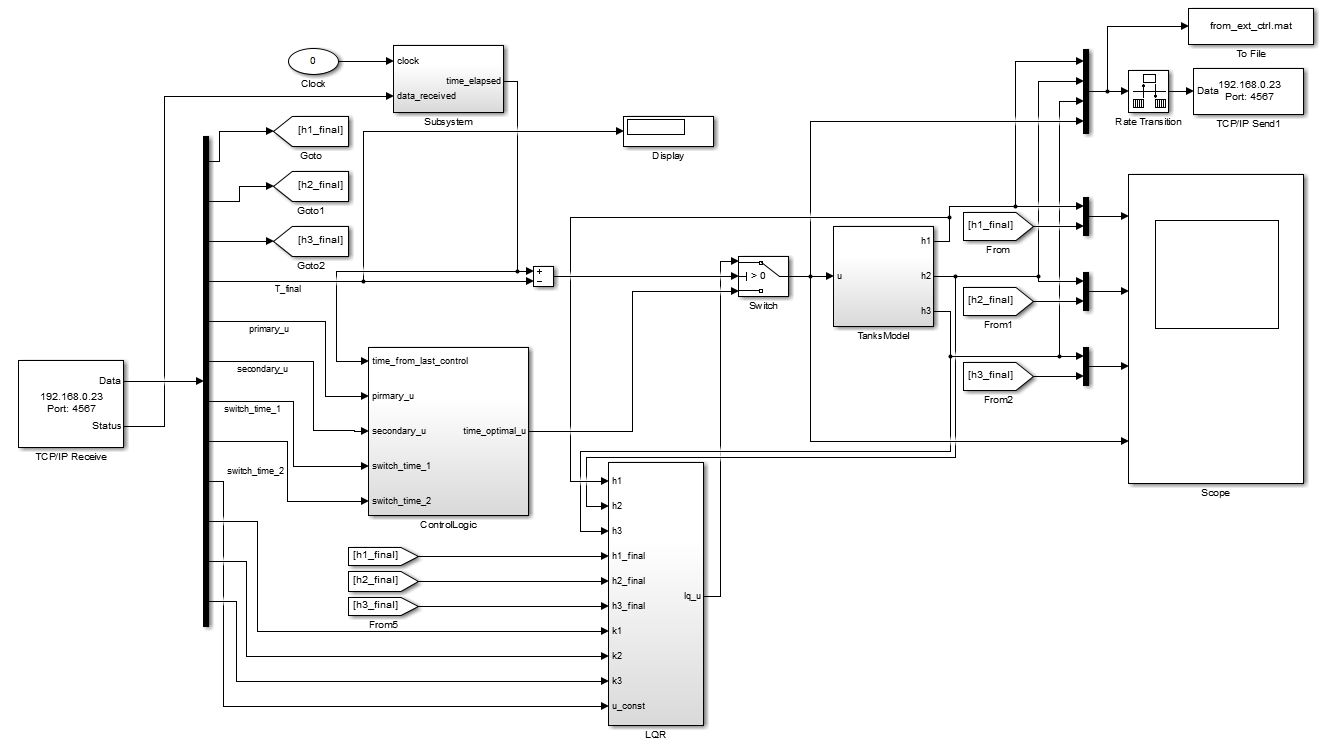
\includegraphics[scale=0.65,angle=90]{Grafika/simulink_model}
    \caption{Model niższego poziomu aplikacji w programie Simulink. Źródło: własne.}
    \label{fig:simulinkmodel}
\end{figure}

Przygotowano model w programie Simulink, pokazany na rys. \ref{fig:simulinkmodel}, który stanowi niższy poziom aplikacji. Zawiera on następujące komponenty:
\begin{itemize}
    \item odbiór danych z wyższego poziomu aplikacji za pomocą protokołu TCP,
    \item układ wyznaczający czas rozpoczęcia realizacji zadania sterowania czasooptymalnego,
    \item układ wyznaczający aktualną wartość sterowania czasooptymalnego na podstawie czasów przełączeń,
    \item układ wyznaczający sterowanie liniowo-kwadratowe,
    \item blok wybierający sterowanie do zaaplikowania w modelu (kryterium przełączenia jest czas będący wartością wskaźnika jakości w zadaniu czasooptymalnym),
    \item podsystem zawierający definicję modelu układu zbiorników,
    \item wysyłanie danych uzyskanych w symulacji (aktualnych poziomów wody w zbiornikach i sterowania) do wyższego poziomu aplikacji i zapisywanie ich do pliku w celu późniejszej analizy,
    \item blok pozwalający na rysowanie wykresów trajektorii systemu w czasie symulacji.
\end{itemize}

Przeprowadzone testy komunikacji między poziomami aplikacji wykazały, że serwer urządzeń systemu Tango Controls, będący wyższym jej poziomem, nie jest w stanie obsłużyć wysyłanych w każdym kroku symulacji danych. Zastosowano więc blok wyzwalający wysyłanie z mniejszą częstotliwością. Dobrano eksperymentalnie wartość 100 ms jako okres wysyłania, ponieważ stwierdzono, że dynamika układu jest stosunkowo wolno zmienna, a więc taki okres nie spowoduje większych błędów w obliczaniu sterowania czasooptymalnego przez część obliczeniową aplikacji.